\section{System Features}
\label{sec:system-features}

In this section, the main features of the components will be discussed, as well as possible features that could be implemented in future releases of the product.
The main functionality needed by each component in order for the project to work will be explained into more detail. \newline
The main use cases of the system components are also provided in each subsection in order to describe how the system will be used by the final user. 

\subsection{Conventions}

The priority of the requirements in Section \ref{sec:system-features} and \ref{sec:non-functional} will be indicated by the keywords \textbf{shall}, \textbf{should} and \textbf{would be nice}:

\begin{itemize}
	\item \textbf{Shall}: Requirements that must be implemented as a minimum; resources must be allocated to these requirements.
	\item \textbf{Should}: Requirements that add more functionality to the software, but are not the core required to work; if possible, resources will be allocated.
	\item \textbf{Would be nice}: Requirements considered good ideas and would be implemented if there are sufficient resources or in later versions of the software.
\end{itemize}


\subsection{Petri net editor}
\label{sec:sf-petrinet}
\writer{Albert}

The Petri net editor is a component that will extend the features provided by the \textit{ePNK}, in order to fulfil the requirements of the project. The extended features include \textit{Input Places} and the definition of links between geometry and animation components.

\subsubsection{Functional Requirements}

\begin{enumerate}
	\item The Petri net editor \textbf{shall} allow the user to create, edit and delete Places.
	\item The Petri net editor \textbf{shall} allow the user to create, edit and delete Tokens inside Places.
	\item The Petri net editor \textbf{shall} allow the user to create, edit and delete Transitions.
	\item The Petri net editor \textbf{shall} allow the user to create, edit and delete Arcs. An arc \textbf{shall} connect a Place to a Transition or vice versa.
	\item The Petri net editor \textbf{shall} allow the user to define a Geometry label to a Place.
	\item The Petri net editor \textbf{shall} allow the user to define an Appearance label to a Place.
	\item The Petri net editor \textbf{shall} allow the user to define an Input Place label to a Place.
	\item The Petri net editor \textbf{shall} allow the user to define an Animation label to a Place.
	\item The Petri net editor \textbf{shall} allow the user to save and load a Petri net model.
	\item The Petri net editor \textbf{shall} create a Petri net file in a format that can be read by the Simulator.
	\item It \textbf{would be nice} that the Petri net editor allowed the user to undo and redo actions.
	\item It \textbf{would be nice} that the Petri net editor allowed the user to copy and paste.
\end{enumerate}

\subsubsection{Use cases}

The features are shown in Figure~\ref{fig:use-cases-petri-net-editor}.

\begin{figure}[htp]
\begin{center}
  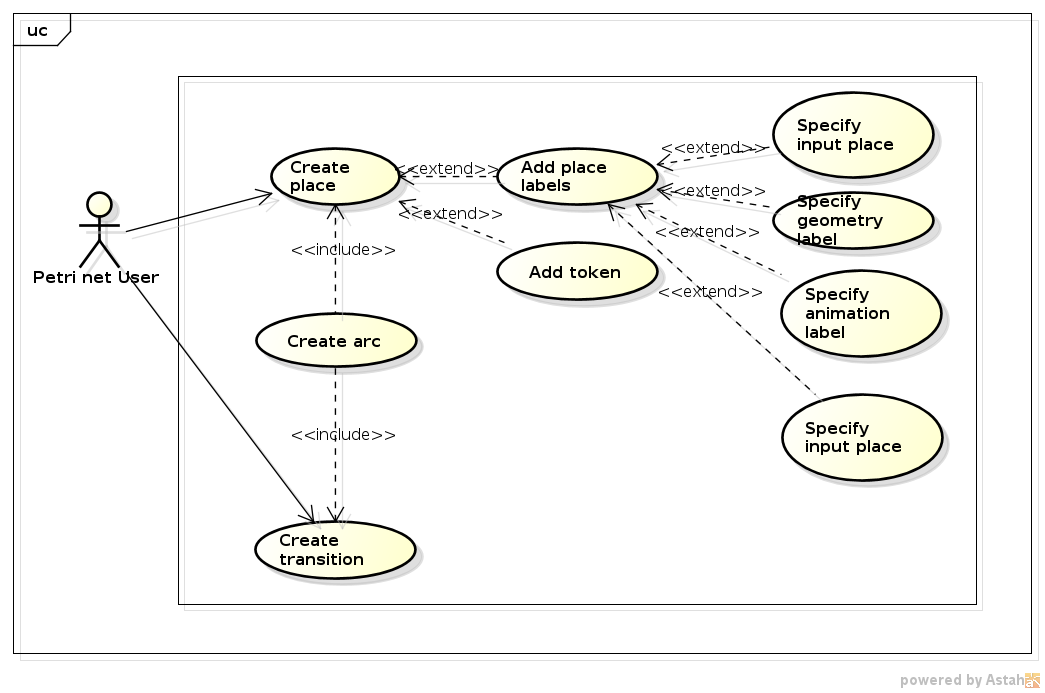
\includegraphics[width=0.8\textwidth]{image/uc-petri-net.png}
  \caption{Use cases for the Petri net Editor}
  \label{fig:use-cases-petri-net-editor}
\end{center}
\end{figure}
\subsection{Geometry editor}
\label{sec:sf-geometry}

Geometry editor is a tool to create and edit geometry. Geometry consists of geometry objects. They are either lines or points. Geometry editor has following requirements.

\subsubsection{Functional Requirements}

\begin{enumerate}
	\item Geometry editor \textbf{shall} allow user to create, edit and delete points.
	\item Geometry editor \textbf{shall} allow user to create, edit and delete define point as inputPoint, Connector or bendPoint.
	\item Geometry editor \textbf{shall} allow user to create, edit and delete lines by using connectors and bendPoints.
	\item Geometry editor \textbf{shall} allow user to load and save geometry file.
	\item Geometry editor \textbf{shall} allow user to define labels for geometry objects.
	\item Geometry editor \textbf{shall} create unique IDs for geometry objects.
	\item Geometry editor \textbf{should} allow user to create parametric curved lines.
	\item Geometry editor \textbf{should} allow user to use undo and redo.
	\item Geometry editor \textbf{should} allow user to use copy, paste and cut geometry objects.
	\item Geometry editor \textbf{should} have a Graphical User Interface.
	\begin{enumerate}
		\item Geometry editor \textbf{should} have drag and drop interface.
		\item Geometry editor \textbf{should} enable editing of geometries with a text input.
		\item It \textbf{would be nice} if the geometry editor allows user to create different kinds of parametric curved lines, such as Catmull-rom spline and Bézier-curves.
		\item It \textbf{would be nice} if the geometry editor allows user to zoom and pan the geometry canvas.
		\item It \textbf{would be nice} if the geometry editor allows user select multiple geometry objects simultaneously.
		\item It \textbf{would be nice} if the geometry editor allows user to load multiple geometries on same canvas.
		\item It \textbf{would be nice} if the geometry editor allows user select multiple geometry objects simultaneously.
		\item It \textbf{would be nice} if the geometry editor allows user to rotate and scale geometry objects.
		\item It \textbf{would be nice} if the geometry editor allows user to toggle visibility of geometry objects while using geometry editor.
	\end{enumerate}
	\item It \textbf{would be nice} if you could specify a Petri ned model from which the geometry is being specified from and it is validated.
\end{enumerate}

\subsubsection{Use cases}

The uses of geometry editor is summed up in the use case diagram in Figure~\ref{fig:use-cases-geometry-editor}.

\begin{figure}[htp]
\begin{center}
  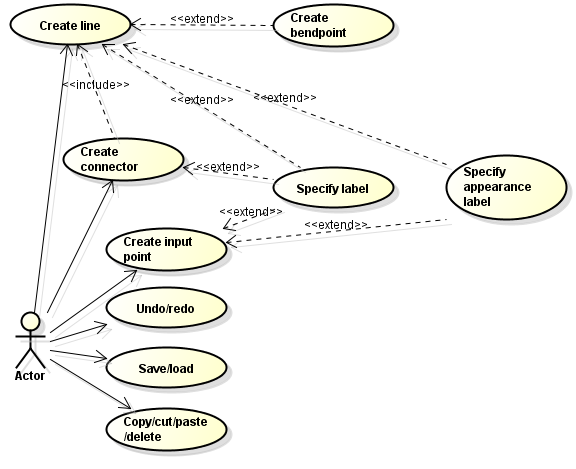
\includegraphics[width=0.5\textwidth]{image/uc-geometry.png}
  \caption{Use cases for the Geometry editor}
  \label{fig:use-cases-geometry-editor}
\end{center}
\end{figure}
\subsection{Appearance Editor}
\label{sec:sf-appearance}

The Appearance Editor is a component that will allow the user to add visual information such as shapes and textures to the Petri net elements to be simulated. The connection between the appearance files and the Petri net elements will be done via the \textit{appearance label}. 

\subsubsection{Functional Requirements}

\begin{enumerate}
\item The Appearance Editor \textbf{shall} allow the user to link appearance labels to 3D objects by choosing a predefined file.
\item The Appearance Editor \textbf{shall} allow the user to link appearance labels to textures by choosing a predefined file.
\item The Appearance Editor \textbf{shall} create an Appearance file in a format that can be read by the Configuration Editor.
\item The Appearance Editor \textbf{shall} allow the user to load an Appearance file.
\item The Appearance Editor \textbf{shall} allow the user to save an Appearance ]file.
\item \textbf{It would be nice} to allow the user to load a Petri net file in order to retrieve all the appearance labels.     
\end{enumerate}

\subsubsection{Use cases}

The features described above are shown in Figure~\ref{fig:use-cases-appearance-editor}.

\begin{figure}[htp]
\begin{center}
  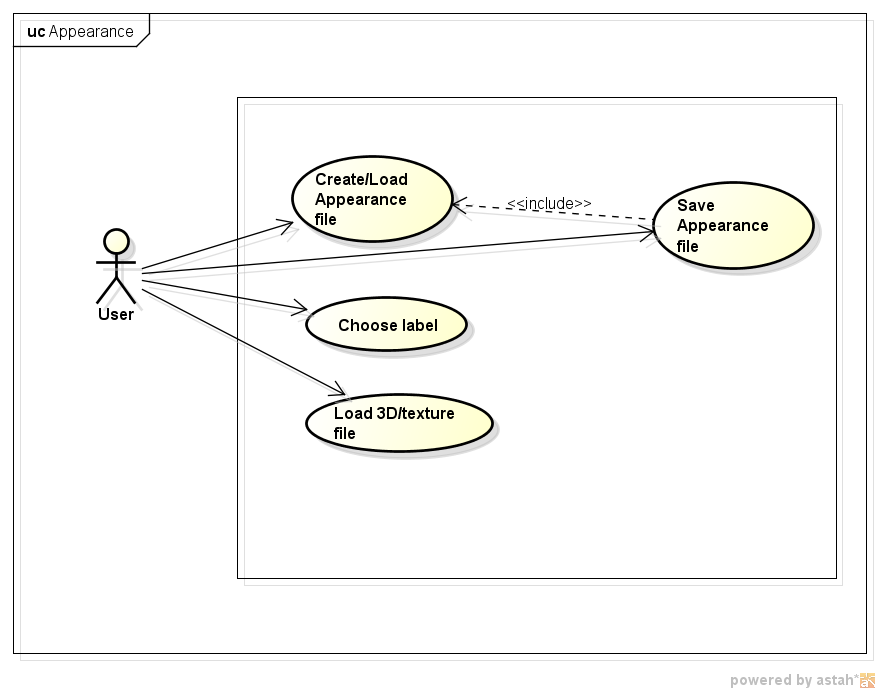
\includegraphics[width=0.8\textwidth]{image/uc-appearance.png}
  \caption{Use cases for the Appearance Editor}
  \label{fig:use-cases-appearance-editor}
\end{center}
\end{figure}


\subsection{Configuration Editor}
\writer{Albert}

The configuration editor is a component that will work as a connector between the Petri net editor (Section \ref{sec:sf-petrinet}), the Geometry editor (Section \ref{sec:sf-geometry}) and the Appearance editor (Section \ref{sec:sf-appearance}). 

\subsubsection{Functional Requirements}

\begin{enumerate}
	\item The configuration editor \textbf{shall} allow the user to input a Petri net file containing its model.
	\item The configuration editor \textbf{shall} allow the user to input a Geometry file containing its model.
	\item The configuration editor \textbf{shall} allow the user to input an Appearance file containing its model.
	\item The configuration editor \textbf{shall} allow the user to start a simulation with the referenced Petri net, Geometry and Appearance models.
	\item It \textbf{would be nice} if the configuration editor allows the user to validate the data.
	\item It \textbf{would be nice} if the configuration editor to save and load a specific configuration to a file.
\end{enumerate}
\subsection{3D Simulator}
\label{sec:sf-simulator}
The functionality of the 3D simulator can be specified using the following statements:
\begin{enumerate}
\item The simulator \textbf{shall} allow the user to play the simulation.
\item The simulator \textbf{shall} allow the user to pause the simulation.
\item The simulator \textbf{shall} allow the user to reset the simulation.
\item The simulator \textbf{shall} allow the user to add tokens on input places.
\item The simulator \textbf{shall} allow the user to exit the simulation.
\item The simulator \textbf{should} allow the user to change the orientation of the view.
\item It \textbf{would be nice} if the simulator allowed the user to take screenshots.
\item It \textbf{would be nice} if the simulator allowed the user to forward the simulation.
\item It \textbf{would be nice} if the simulator allowed the user to rewind the simulation.
\end{enumerate}